% !TeX spellcheck = fr_FR
\documentclass[aspectratio=169,utf8]{beamer}

\usepackage[french]{babel}
\usepackage{color}
\usepackage{listings}
\definecolor{mygreen}{rgb}{0,0.6,0}
\definecolor{mygray}{rgb}{0.47,0.47,0.33}
\definecolor{myorange}{rgb}{0.8,0.4,0}
\definecolor{mywhite}{rgb}{0.98,0.98,0.98}
\definecolor{myblue}{rgb}{0.01,0.61,0.98}
\lstset{%
  language=c++,
  numbers=left,
  numbersep=1em,
  backgroundcolor=\color{mywhite},
  numberstyle=\tiny\color{mygray},
  basicstyle=\footnotesize\ttfamily,
  stringstyle=\color{red},
  commentstyle=\color{mygray},
  deletekeywords={...},
  escapeinside={\%*}{*)},
  extendedchars=true,
  keywordstyle=\color{myorange},
  morekeywords={*,...},
  rulecolor=\color{black},
  rulesepcolor=\color{myblue},
  stringstyle=\color{myorange},
  tabsize=2
}
\usepackage{url}

\title{Objets connectés}
\author{François Roland}
\date{2 novembre 2018}


\begin{document}
\frame{\titlepage}

\begin{frame}
  \frametitle{Partage d'informations}
  \begin{center}
    \url{http://bit.ly/iot3d}
  \end{center}
\end{frame}

\begin{frame}
  \frametitle{Plan}
  \tableofcontents
\end{frame}

\section{Introduction}

\begin{frame}
  \frametitle{Règles de conduite}
  Horaire
  \begin{itemize}
    \item 8:30 -- 12:30 (pause vers 10:30)
    \item 13:30 -- 17:30 (pause vers 15:30)
  \end{itemize}
  Prise de parole
  \begin{itemize}
    \item Questions et commentaires bienvenus 
    \item Parler suffisamment fort pour l'ensemble du groupe
    \item Ne pas monopoliser la parole
    \item Ne pas interrompre
  \end{itemize}
  Respect de chacun
  \begin{itemize}
    \item Commentaires discriminatoires non tolérés
    \item Ne pas perturber le cours (gsm, réseaux sociaux)
  \end{itemize}
\end{frame}

\begin{frame}
  \frametitle{François Roland}
  \begin{columns}
    \begin{column}{.3\textwidth}
      \begin{center}
        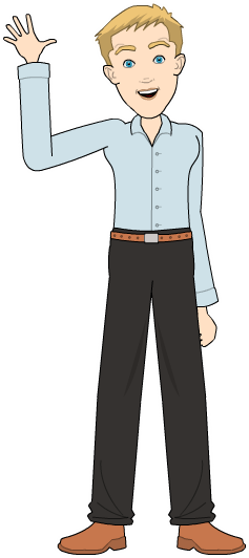
\includegraphics[height=.7\textheight]{francois1.png}
      \end{center}
    \end{column}
    \begin{column}{.7\textwidth}
      Ingénieur Civil en Informatique et Gestion \\
      Aujourd'hui \\
      \begin{itemize}
        \item Chercheur Télécoms UMONS
        \item Chargé de projet Fab-IoT-Lab au FabLab Mons
        \item Indépendant complémentaire
      \end{itemize}
      Dans le passé \\
      \begin{itemize}
        \item Consultant en développement logiciel
        \item Take-Eat-Easy (startup)
      \end{itemize}
    \end{column}
  \end{columns}
\end{frame}

\begin{frame}
  \frametitle{François Roland}
  \begin{columns}
    \begin{column}{.3\textwidth}
      \begin{center}
        
\includegraphics[height=.7\textheight]{francois2.png}
      \end{center}
    \end{column}
    \begin{column}{.7\textwidth}
      Électronique \\
      Programmation \\
      Conception mécanique \\
      Enseignement
    \end{column}
  \end{columns}
\end{frame}

\begin{frame}
  \frametitle{Et vous ?}
  \begin{columns}
    \begin{column}{.4\textwidth}
      Prénom \\
      Attentes \\
      Compétences IoT
      \begin{itemize}
        \item Programmation
        \item Électronique
        \item Télécommunications
      \end{itemize}
      Projets personnels IoT
    \end{column}
    \begin{column}{.6\textwidth}
      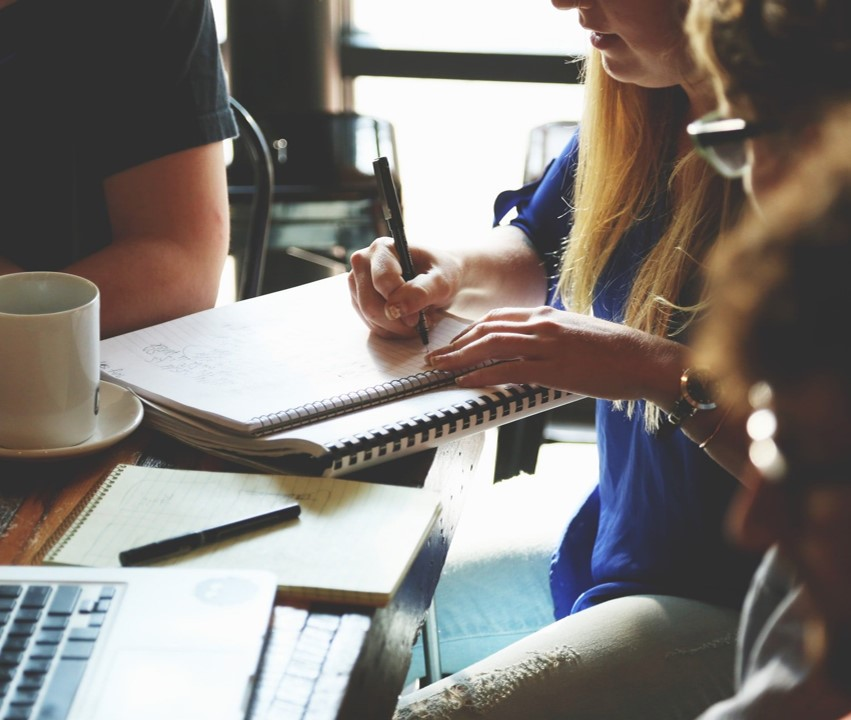
\includegraphics[width=\textwidth]{etvous.jpg}
    \end{column}
  \end{columns}
\end{frame}

\section{Jours 1 et 2}
\subsection{Qu'est-ce que l'IoT ?}

\begin{frame}
  \frametitle{Qu’est-ce que l’Internet des Objets ?}
  \begin{columns}
    \begin{column}{.8\textwidth}
      \begin{quotation}
        <<~L'Internet des objets, ou IdO (en anglais Internet of Things, ou IoT), est l'extension d'Internet à des choses et à des lieux du monde physique.
          
        Alors qu'Internet ne se prolonge habituellement pas au-delà du monde électronique, l'Internet des objets connectés représente les échanges d'informations et de données provenant de dispositifs du monde réel avec le réseau Internet.~>>
      \end{quotation}
    \end{column}
    \begin{column}{.2\textwidth}
      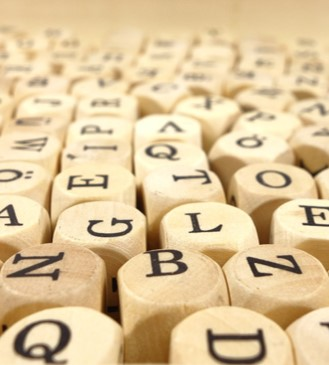
\includegraphics[width=\textwidth]{definition.jpg}
    \end{column}
  \end{columns}

  \hfill{\scriptsize\url{https://fr.wikipedia.org/wiki/Internet_des_objets}}
\end{frame}

\begin{frame}
  \frametitle{Qu'est-ce qu'un objet connecté ?}
  \begin{columns}
    \begin{column}{.4\textwidth}
      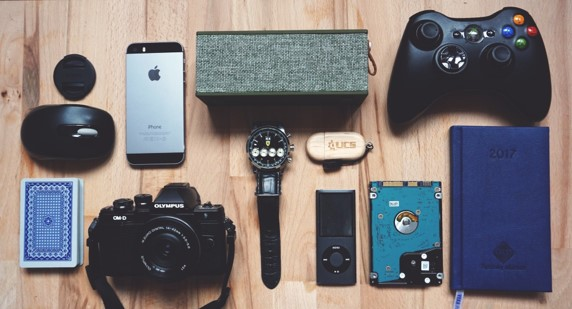
\includegraphics[width=\textwidth]{objetsconnectes.jpg}
    \end{column}
    \begin{column}{.6\textwidth}
      Un objet connecté est constitué de :
      \begin{itemize}
        \item Un capteur ou actionneur pour interagir avec son environnement
        \item Un micro-contrôleur pour transformer les données
        \item Un moyen de communication pour communiquer avec le monde
        \item Une source d’énergie pour alimenter les éléments précédents
      \end{itemize}
    \end{column}
  \end{columns}
\end{frame}

\begin{frame}
  \frametitle{Histoire de l'IoT}
  \begin{columns}
    \begin{column}{.3\textwidth}
      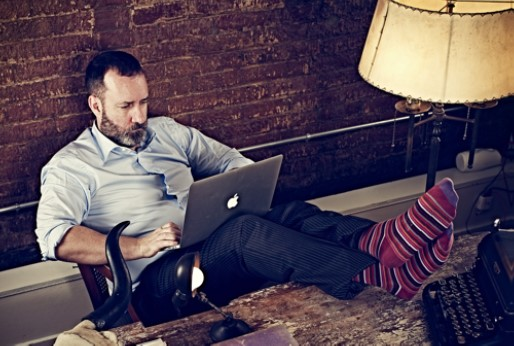
\includegraphics[width=\textwidth]{kevinashton.jpg}
    \end{column}
    \begin{column}{.7\textwidth}
      L’histoire des objets connectés débute en \emph{1999} lorsque Kevin Ashton, pionnier de la technologie \emph{RFID} (Radio Frequency IDentification – Technologie d’identification automatique), invente l’expression <<~\emph{Internet des Objets}~>>.

      Cette même année, le concept naît aux États-Unis et particulièrement au \emph{MIT} (Massachusetts Institute of Technology).
      Ce laboratoire est dédié à la création d’objets connectés à l’aide de l’identification par radiofréquence et les réseaux de capteurs sans fil.
    \end{column}
  \end{columns}
\end{frame}

\begin{frame}
  \frametitle{Histoire de l'IoT}
  \begin{columns}
    \begin{column}{.3\textwidth}
      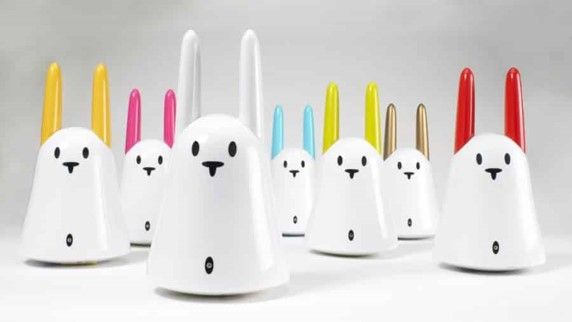
\includegraphics[width=\textwidth]{nabaztag.jpg}
    \end{column}
    \begin{column}{.7\textwidth}
      En \emph{2003}, Rafi Haladjian, inventeur du premier opérateur Internet en France (Francenet), créé la \emph{lampe DAL}. Une lampe d’ambiance équipée de 9 LEDs, proposant différentes couleurs et commercialisée à \emph{790 euros}.

      Deux ans plus tard, l’entreprise du créateur lance le \emph{Nabaztag}, un lapin connecté en WiFi qui lit les mails à haute voix, émets des signaux visuels et diffuse de la musique.
    \end{column}
  \end{columns}
\end{frame}

\begin{frame}
  \frametitle{Histoire de l'IoT}
  \begin{columns}
    \begin{column}{.3\textwidth}
      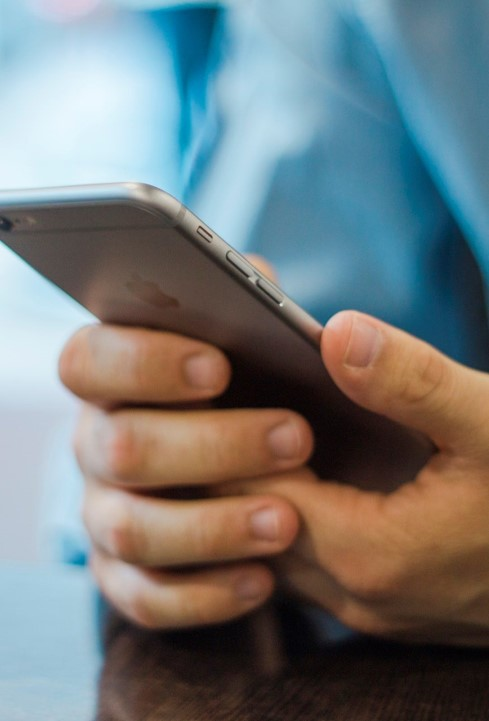
\includegraphics[width=\textwidth]{smartphone.jpg}
    \end{column}
    \begin{column}{.7\textwidth}
      C’est néanmoins en \emph{2007} que le phénomène de l'IoT a pris de l’ampleur, avec la démocratisation des \emph{smartphones} et la sortie du premier iPhone par Apple.
      La dématérialisation est en marche.

      Nous vivons actuellement une rupture forte.
      Celle nous permettant de connecter Internet au moindre objet de notre quotidien.
      Ces objets génèrent une quantité de données telle que ses perspectives d’exploitation semblent sans limite.

      Le sujet des data suscite des questions éthiques délicates sur le respect de la vie privée.
    \end{column}
  \end{columns}
\end{frame}


\subsection{Arduino}

\begin{frame}
  \frametitle{Arduino}
  \begin{center}
    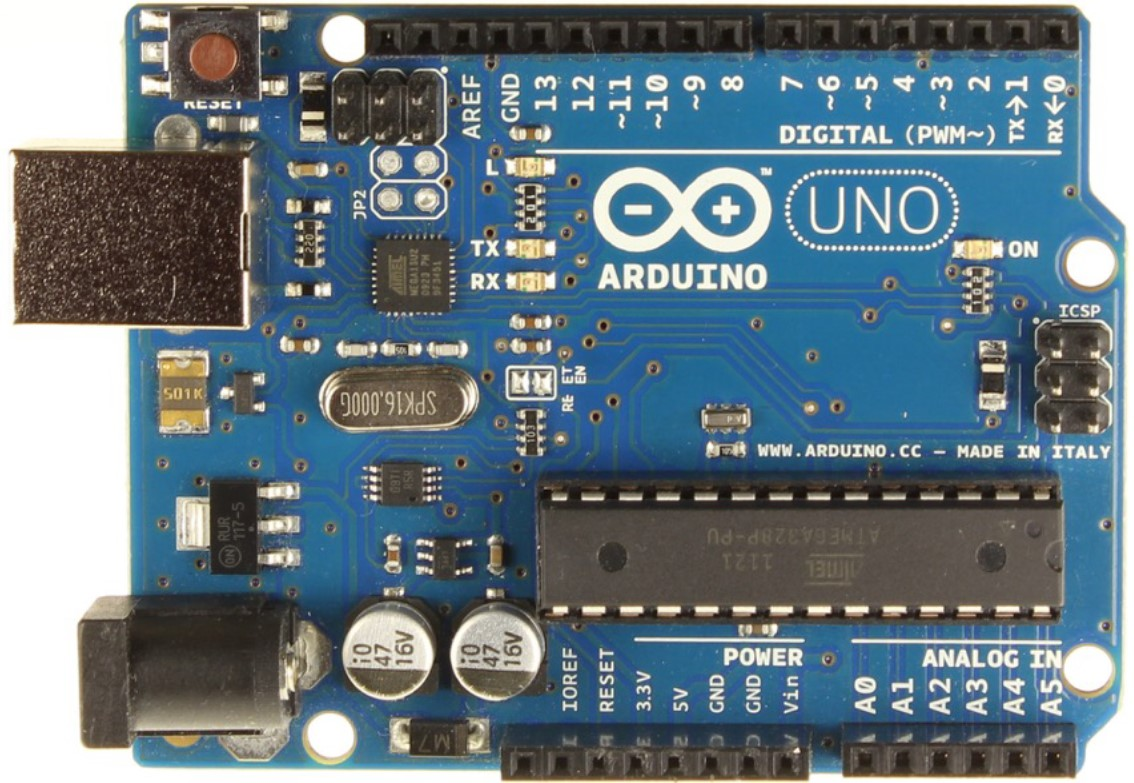
\includegraphics[height=.8\textheight]{arduino.jpg}
  \end{center}
\end{frame}

\begin{frame}[fragile]
  \frametitle{Programmation C pour Arduino}
  \begin{lstlisting}
Code == texte;
Exécution ligne par ligne;
// Commentaire
  \end{lstlisting}
\end{frame}

\begin{frame}[fragile]
  \frametitle{Variable}
  \begin{columns}
    \begin{column}{.4\textwidth}
      \begin{lstlisting}
int pin = 13;
      \end{lstlisting}
    \end{column}
    \begin{column}{.6\textwidth}
      \begin{itemize}
        \item Un type
        \begin{itemize}
          \item \lstinline{int}
          \item \lstinline{float}
          \item \lstinline{char[]}
        \end{itemize}
        \item Un nom
        \item Une valeur de départ (\emph{optionnel})
      \end{itemize}
    \end{column}
  \end{columns}
\end{frame}

\begin{frame}[fragile]
  \frametitle{Fonction}
  \begin{columns}
    \begin{column}{.6\textwidth}
      \begin{lstlisting}
int myMultiplyFunction(int x, int y) {
  return x * y;
}

void loop() {
  int k = myMultiplyFunction(2, 3);

  Serial.println(k); // 6
}
      \end{lstlisting}
    \end{column}
    \begin{column}{.4\textwidth}
      \begin{itemize}
        \item Un nom
        \item Des paramètres (\emph{optionnel})
        \item Un type de retour
        \item Un code d’implémentation
      \end{itemize}
    \end{column}
  \end{columns}
\end{frame}

\begin{frame}[fragile]
  \frametitle{Fonction}
  \begin{lstlisting}
void setup() {
  ...
}
  \end{lstlisting}
  Est exécuté une seule fois au démarrage.

  \begin{lstlisting}[firstnumber=4]
void loop() {}
  ...
}
  \end{lstlisting}
  Est exécuté en boucle après \lstinline|setup()|.
\end{frame}

\begin{frame}[fragile]
\frametitle{Condition}
\begin{columns}
  \begin{column}{.5\textwidth}
    \begin{lstlisting}
if (x > 120) {
  digitalWrite(LEDpin1, HIGH);
  digitalWrite(LEDpin2, HIGH);
}

if (y == 150) {
  digitalWrite(LEDpin4, LOW);
} else {
  digitalWrite(LEDpin4, HIGH);
}
    \end{lstlisting}
  \end{column}
  \begin{column}{.5\textwidth}
    \begin{itemize}
      \item Une condition à tester
      \item Un bout de code à exécuter si la condition est vérifiée
      \item Un bout de code à exécuter si la condition n’est pas vérifiée (\emph{optionnel})
    \end{itemize}
  \end{column}
\end{columns}
\end{frame}

\begin{frame}[fragile]
  \frametitle{Boucle \lstinline{for}}
  \begin{columns}
    \begin{column}{.5\textwidth}
      \begin{lstlisting}
for (int i=0; i <= 255; i++) {
  analogWrite(PWMpin, i);
  delay(10);
}
      \end{lstlisting}
    \end{column}
    \begin{column}{.5\textwidth}
      À utiliser quand on sait combien de fois il faut répéter la boucle.
      \begin{itemize}
        \item Un compteur
        \item Un bout de code à répéter
      \end{itemize}
    \end{column}
  \end{columns}
\end{frame}

\begin{frame}[fragile]
  \frametitle{Boucle \lstinline{while}}
  \begin{columns}
    \begin{column}{.5\textwidth}
      \begin{lstlisting}
int value = 0;
while(value < 10) {
  digitalWrite(LEDpin3, HIGH);
  delay(200);
  digitalWrite(LEDpin3, LOW);
  value = analogRead(TRIMpin);
}
      \end{lstlisting}
    \end{column}
    \begin{column}{.5\textwidth}
      À utiliser lorsque l’on veut répéter une boucle tant qu’une condition est vérifiée
      \begin{itemize}
        \item Une condition à vérifier
        \item Un code à répéter
      \end{itemize}
    \end{column}
  \end{columns}
\end{frame}

\subsection{Découvrons les kits}

\begin{frame}
  \frametitle{Découvrons les kits}
\end{frame}

\subsection{Passons à la pratique}

\begin{frame}
  \frametitle{Passons à la pratique}
\end{frame}

\section{Jour 3}

\subsection{Communications sans fil}

\begin{frame}
  \frametitle{Communications sans fil}
\end{frame}

\subsection{Outils de développement IoT}

\begin{frame}
  \frametitle{Outils de développement IoT}
\end{frame}

\section{Conclusion}

\begin{frame}
  \frametitle{Conclusion}
\end{frame}

\end{document}
